\section{工厂生产计划扩展(问题二)} % (fold)
\label{sec:工厂生产计划扩展}

现实情况中,新采购的组件并不能直接投入使用,而是应由供应商生产、交付、转运至库存中,再供生产取用。
因此,在生产工厂发出采购订单后,订购的组件需经过一定延迟时间,才能供实际生产使用。

\subsection{模型的建立与求解} % (fold)
\label{sub:模型的建立与求解}

% subsection 模型的建立与求解 (end)

本题要求在记入组件入库延迟的前提下,设计生产工厂每周7天的生产计划。
与问题一组件入库无延迟不同,问题二中组装产品所需的组件要提前一天入库才能参与生产。

在此基础上,由于该工厂第一天(周一)开始时没有任何组件库存,而新采购的组件在第二天(周二)才能投入生产,在第三天(周三)才可生产出WPCR。因此工厂必须在前一天(上周周日),准备好了刚好满足周一需求的WPCR库存(即$y_0^{\text{WPCR}} = 39+36=75$),以免缺货断供。

综上,本文在问题一模型基础上,添加以下约束条件:
\begin{equation}\label{新条件}
	\eta_{r^{\prime}}^{r} x_{t}^{r^{\prime}} \leqslant y_{t-1}^{r},\quad t=1,2, \cdots, T, r=1,2, \cdots, R.
\end{equation}
上式中,通过令工厂当天生产所需组件数量$\eta_{r^{\prime}}^{r} x_{t}^{r^{\prime}}$,小于前一天库存组件$y_{t-1}^{r}$,以限制工厂只得使用前一天的组件库存生产新组件。

将上式\ref{新条件}加入问题一中线性规划模型式\ref{总模型},得:

\begin{equation}\label{二模型}
	\begin{aligned}
&\min \quad z  = \sum_{t  = 1}^{T} \sum_{r = 1}^{R}\left(s^{r} \omega_{t}^{r}+h^{r} y_{t}^{r}\right)\\
& \ \begin{array}{r@{\quad}l@{}l@{\quad}l}
\mathrm{s.t. } 	&\sum_{r=1}^{R} M_{t}^{r} \leqslant M_{t}; &\\
&M_{t}^{r} \leqslant M_{t}^{r} \omega_{t}^{r}, &t=1,2, \cdots, T, r=1,2, \cdots, R;\\
& y_{t}^{r}=y_{t-1}^{r}+x_{t}^{r}-\eta_{r}^{r} x_{t}^{r^{\prime}}, &t=1,2, \cdots, T,  r=1,2, \cdots, R; \\
&\omega_{t}^{r} \in\{0,1\}, &t=1,2, \cdots, T, r=1,2, \cdots, R; \\
&x_{t}^{r}=x_{t}^{r} \omega_{t}^{r},&t=1,2, \cdots, T, r=1,2, \cdots, R;\\
&c^{r} x_{t}^{r}=M_{t}^{r} \omega_{t}^{r}, &t=1,2, \cdots, T, r=1,2, \cdots, R; \\
&M_{t}^{r} \geqslant 0,& r=1,2, \cdots, R ;\\
&y_{0}^{r}=y_{T}^{r}=0,& r=1,2, \cdots, R ;\\
&x_{t}^{r}, y_{t}^{r} \geqslant 0, &t=1,2, \cdots, T, r=1,2, \cdots, R;\\
&y_{t-1}^{\mathrm{WPCR}}+x_{t}^{\mathrm{WPCR}}-y_{t}^{\mathrm{WPCR}}=d_{t}, & t=1,2, \cdots, T; \\
&\eta_{r^{\prime}}^{r} x_{t}^{r^{\prime}} \leqslant y_{t-1}^{r}, &t=1,2, \cdots, T, r=1,2, \cdots, R;
\end{array}.
\end{aligned}
\end{equation}

在式\ref{二模型}中,$t = 1, 2,\cdots, 210.$ 特别地,当$t = 1, 2,\cdots, 5$时,定义$\mu_{-4}=\mu_{-3}=\mu_{-2}=\mu_{-1}=\mu_{0}=0$.
在安排检修时, 如果希望问题2的生产计划保持不变, 可以看出: 根据问题2的结果, 有多天无生产计划,因此可以安排检修;究竟将检修安排在哪天呢?
实际上,由于检修后生产能力发生变化,把检修安排在本身没有生产任务的时段不一定是最佳的.
从题目给的条件来看,将检修安排在任何一天都是可以的. 因此模型引入了0—1变量,但以上模型由于规模较大,求解很慢.
所以本文并未得到全局最优解,而是在有限时间内寻找了局部最优解.
直观来看,周一的生产总工时限制宽、周六检修难以满足外部WPCR需求,所以检修不应安排在这两天.
为了降低库存成本,可以在其余时间中选择WPCR较少的七天作为起点,再通过启发式优化算法求解以上问题,这是本题的另一种解题思路.
但本文认为与线性规划相比,其缺乏确定的全局最优解,因此本文最终未选用该方法.
2
\subsection{生产方案展示} % (fold)
\label{sub:生产方案展示}


\begin{table}[!htbp]
\centering
\caption{问题二的结果}
\resizebox{\linewidth}{!}{
\begin{tabular}{ccccccccccccccc}
\toprule
\diagbox{日期}{部件(花费)} & WPCR & B   & A   & C   & B2   & B1   & A2        & A3        & A1   & C1   & C2   & C3    & 生产准备费用 & 生产库存费用                \\
\midrule
周一                   & 0    & 0   & 0   & 0   & 624  & 312  & 1872      & 468       & 1404 & 1560 & 390  & 2340  & 500    & 32472                 \\
周二                   & 0    & 156 & 234 & 195 & 1216 & 608  & 0         & 0         & 0    & 1560 & 390  & 2340  & 810    & 22025.5               \\
周三                   & 39   & 304 & 0   & 195 & 0    & 0    & 888       & 222       & 666  & 2800 & 700  & 4200  & 900    & 30752.5               \\
周四                   & 39   & 0   & 111 & 350 & 1168 & 584  & 1752      & 438       & 1314 & 0    & 0    & 0     & 870    & 23669                 \\
周五                   & 37   & 292 & 219 & 0   & 0    & 0    & -2.84E-14 & -7.11E-15 & 0    & 1600 & 400  & 2400  & 690    & 13956.5               \\
周六                   & 33   & 0   & 0   & 200 & 0    & 0    & 0         & 0         & 0    & 0    & 0    & 0     & 420    & 820                   \\
周天                   & 40   & 0   & 0   & 0   & 0    & 0    & 0         & 0         & 0    & 0    & 0    & 0     & 240    & 0                     \\
\cline{14-15}
总和                   & 188  & 752 & 564 & 940 & 3008 & 1504 & 4512      & 1128      & 3384 & 7520 & 1880 & 11280 & \multicolumn{2}{c}{128125.5~}  \\
\bottomrule
\end{tabular}
}
\end{table}

\begin{figure}[!htbp]
	\centering
	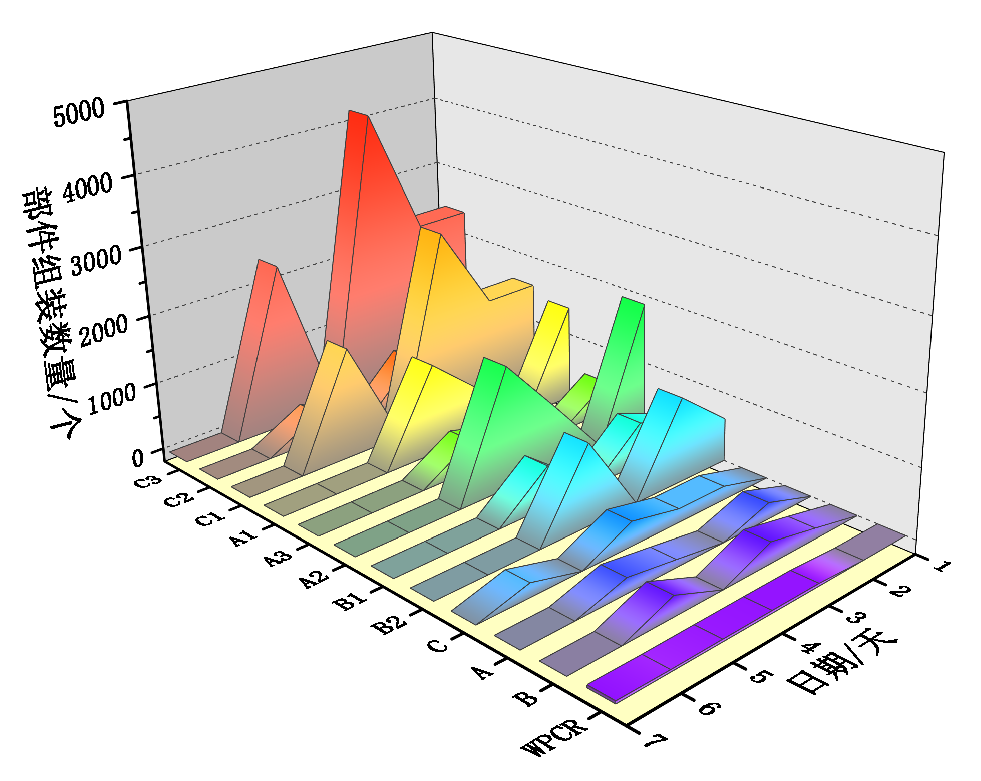
\includegraphics{Image/问题二展示.eps}
	\caption{每日组件组装数量}\label{每日组件组装数量}
\end{figure}

\begin{figure}[!htbp]
	\centering
	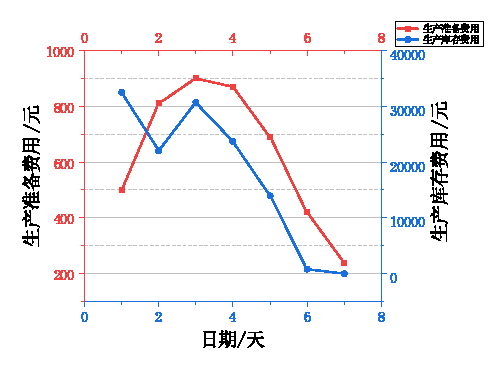
\includegraphics{Image/问题二展示2.eps}
	\caption{每日成本费用}\label{每日成本费用}
\end{figure}

\begin{figure}[!htbp]
	\centering
	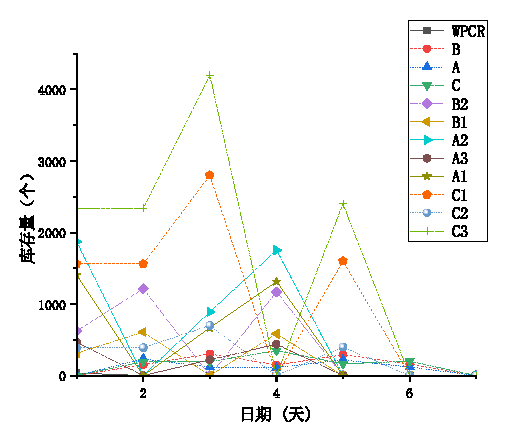
\includegraphics{Image/问题二库存.eps}
	\caption{每日库存数量}\label{每日库存数量}
\end{figure}

问题2要求必须使用前一天的库存进行当日的生产工作,此时:开车型将每天生产当日所需的WPCR、次日所需的关键组件和再次一天所需的其余组件,其中后两项即为库存;仓储型则会将集中生产WPCR、在前一天生产关键组件并在再前一天生产所需的其余组件,形成共三天的生产计划.
但这两种计划的库存费用相等、则仓储型由于节约了大量生产准备费而占据优势,问题2的条件明显对仓储型有利.

由图3可知,工厂前期生产较多、后期较少,这是仓储型的特点.
由图4可知,WPCR库存量始终几乎为0,体现了开车型的特点.
和问题1不同,在问题2中工厂对仓储型和开车型策略都未表现出明显的倾向性,可以说问题2的额外要求和昂贵的仓储成本都是工厂生产计划的制订需要考虑的关键因素.

% subsection 生产方案展示 (end)
% section 工厂生产计划扩展 (end)
